\documentclass[10pt,letterpaper,twoside]{article}
\usepackage[latin1]{inputenc}
\usepackage[pdftex]{graphicx}     % Add some packages for figures. Read epslatex.pdf on ctan.tug.org
\usepackage{geometry}
\usepackage{fancyhdr}
\usepackage{amsmath}
\usepackage{amsfonts}
\usepackage{bm}
\usepackage{outlines}
\usepackage{calligra}
\usepackage{pxfonts}
%\usepackage[T1]{fontenc}{pxfonts}
%\usepackage{newpxtext,newpxmath}
\usepackage{mathrsfs}
\usepackage{units}
\usepackage{amssymb}
\usepackage{titlesec}
\usepackage[section]{placeins}
\usepackage{color}
\usepackage[activate={true,nocompatibility},final,tracking=true,kerning=true,spacing=true,factor=1200,stretch=40,shrink=40]{microtype}
\usepackage[colorlinks=true,
			linkcolor=webgreen, %defined below
			filecolor=webbrown, %defined below
			citecolor=webgreen, %defined below
			%------------- Doc Info ---------------------------------
			pdftitle={Notes and tips from PHYS 211},
			pdfauthor={J. L. Lanfranchi},
			pdfsubject={},
			pdfkeywords={},
			%------------ Doc View ----------------------------------
			bookmarksopen=true,
			pdfpagemode=UseOutlines]{hyperref}
\definecolor{mygreen}{rgb}{0,0.6,0}
\definecolor{mygray}{rgb}{0.5,0.5,0.5}
\definecolor{mymauve}{rgb}{0.58,0,0.82}
\definecolor{webgreen}{rgb}{0.0,0,0.8}
\definecolor{webgreen}{rgb}{0.0,0,0.8}
\definecolor{webbrown}{rgb}{0,0,0.8}

\setlength{\floatsep}{0.01in}
\setlength{\textfloatsep}{0.01in}
\setlength{\topmargin}{0.01in}
\setlength{\topskip}{0.01in}
\setlength{\textheight}{0.1in}
\setlength{\intextsep}{3pt}

\newcommand{\sectionlinetwo}[2]{%
  \nointerlineskip \vspace{.5\baselineskip}\hspace{\fill}
  {\resizebox{0.5\linewidth}{1.2ex}
    {\pgfornament[color = #1]{#2}
    }}%
    \hspace{\fill}
    \par\nointerlineskip \vspace{.5\baselineskip}
  }

\author{J. L. Lanfranchi}
\title{Notes and Tips Stemming from Intro. Mechanics Labs \& Activities}
\geometry{top=0.55in,left=0.75in,right=0.75in,bottom=0.75in}
\begin{document} 
\vspace{-40pt}
\maketitle
\vspace{-50pt}
\section{Vectors}
\subsection{Notation}
A vector is denoted (when hand writing equations) by an arrow on top of the name: $\vec F$ denotes a vector force and $\vec a$ denotes a vector acceleration.
Textbooks and typeset work frequently use boldface to indicate a vector: $\mathbf F$ and $\mathbf a$.

If you see a boldface letter in an assignment or in the book, \textit{write it down on your paper with an arrow on top}.
It is a vector, not a scalar.
There's a big difference between the two, as you'll grow to appreciate the more you work with each side-by-side.

\subsection{Unit Vectors}
Unit vectors are used to define the directions of a coordinate system.
They are an exception to the arrow-on-top-of-vectors rule, as they are written with ``hats'' on top: $\hat\imath$, $\hat\jmath$, and $\hat k$.

Unit vectors are of unit length (that means their \textbf{length is one}, \textit{not} that they have units).
Confusion can result if you don't realize this when you're working with unit vectors, so remember: Unit vectors \textit{do not have units}.\footnote{
To see that unit vectors do not have units, look at the definition: a unit vector is given by dividing a vector by its magnitude (or length, if you're thinking in distances).
Both the vector and its magnitude carry the same units, so units cancel.
For example, if you have a vector $\vec r$ which represents a displacement, then the units of $\vec r$ are meters and the units of $\left\lVert \vec r\right\rVert $ are meters.
The unit vector associated with it, $\hat r\equiv \frac{\vec r}{\left\lVert \vec r\right\rVert }$, points in the same direction as $\vec r$, has length one, and has \textit{no units}.

%Hopefully a thing without units (a unit vector) that is used to multiply a thing with units (a component of a vector) isn't too hard to deal with: You do something similar every time you double a length, for example.
%Twice five meters is the same as saying $(\unit[5]{m})\times 2$.
%The 2 in that equation has no units.
%Likewise, ``$\unitfrac[17]{m}{s}$ in the horizontal direction'' is written as $\unitfrac[17]{m}{s}$ multiplying the $\hat\imath$ unit vector, or simply $(\unitfrac[17]{m}{s})\,\hat\imath$.
}

\subsection{Components}
The components of a vector are the scalar lengths that contribute to the vector in each coordinate direction.
For example, you could write a vector force in a 3D coordinate system as
$$\vec F = F_x\hat\imath + F_y\hat\jmath + F_z \hat k$$
which has as its \textit{components}
\begin{gather*}
  F_x, \; F_y,\text{ and } F_z.
\end{gather*}
That's it.
No unit vectors are included in this list, no arrows on top; just scalars.
What is the $z$-component of this force? It's $F_z$.
What's the $y$-component of the force? $F_y$.

You might be familiar with the following way of listing the components of a vector:
$$ \left(F_x,\,F_y,\,F_z\right) $$
which is just like specifying the three coordinates of a point, like $(3, -4, 10)$.
That might help keep it straight in your mind that the components of a vector are just simple scalar numbers.

Each component of a vector has the same units as the vector itself.
In the case of force, for example, the components in each of the three directions individually carry units of newtons.

Finally, a vector equation like $\vec F = m\vec a$ can be translated into separate equations that only involve the components of the vectors.
It might seem simple, but I'll write this out explicitly so you see how the separate equations come about, and why there are no vectors left over in the end.
\begin{align*}
  \vec F &= m\vec a \\
  F_x\hat\imath + F_y\hat\jmath + F_z\hat k &= m\left(a_x\hat\imath + a_y\hat\jmath + a_z\hat k \right) \\
  F_x\hat\imath + F_y\hat\jmath + F_z\hat k &= ma_x\hat\imath + ma_y\hat\jmath + ma_z\hat k.
\end{align*}
Because the $\hat\imath$, $\hat\jmath$, and $\hat k$ directions are \textit{orthogonal} to (or independent of) one another, the only way for the equality to hold is if the parts in each direction are independently equal.

This can is demonstrated by projecting the above equation onto each of the coordinate directions.
Mathematically, projection onto each direction means taking the dot (or inner) product with each of the unit vectors.
The dot product has the property that $\hat\imath\cdot\hat\imath=1$, $\hat\jmath\cdot\hat\jmath=1$, and $\hat k\cdot\hat k=1$ while $\hat\imath\cdot\hat\jmath=0$, $\hat\imath\cdot\hat k=0$, etc.
\begin{align*}
  \left(F_x\hat\imath + F_y\hat\jmath + F_z\hat k\right)\cdot\hat\imath &= \left(ma_x\hat\imath + ma_y\hat\jmath + ma_z\hat k\right)\cdot\hat\imath \\
  F_x\,\hat\imath\cdot\hat\imath + F_y\,\hat\jmath\cdot\hat\imath + F_z\,\hat k\cdot\hat\imath &= ma_x\,\hat\imath\cdot\hat\imath + ma_y\,\hat\jmath\cdot\hat\imath + ma_z\,\hat k\cdot\hat\imath \\
  F_x\cdot1 + F_y\cdot0 + F_z\cdot0 &= ma_x\cdot1 + ma_y\cdot0 + ma_z\cdot0 \\
  F_x &= ma_x.
\end{align*}
There are \textit{no} vector bits left over once we've performed the projection.
The last equation above is a restatement of Newton's second law for the $x$-components.
Performing the projection instead in the $\hat\jmath$ and $\hat k$ directions gives the other two component equations, and I record all three below for reference.
\begin{align*}
  F_x &= ma_x,&  F_y &= ma_y,& F_z &= ma_z
\end{align*}

\subsection{Magnitude}
The magnitude of a vector is denoted either by $\left\lVert \vec F\right\rVert $ or by omitting the arrow on top: $F$.
Some use $\left|\vec F\right|$ to denote the magnitude of a vector, but from now on I will try to reserve that $\left| x \right|$ for the absolute value of numbers (this includes complex numbers, where it's called the modulus) so you know what kind of thing is being measured by the notation.
The definition of the magnitude of a vector is
$$F\equiv\left\lVert \vec F\right\rVert  \equiv \sqrt{F_x^2 + F_y^2 + F_z^2}$$
and this value is \textit{always greater than or equal to zero}. This is an important point to remember when writing the components of a vector in terms of its magnitude.

You'll note that because each of the vector's components carry the same units as the vector, the above equation points back to the fact that the magnitude of the vector also carries those same units.
It makes sense, but it's a good consistency check on which parts of the vector we said have units (the components) and which don't have units (the unit vectors).

\subsection{Assigning signs}
\subsubsection{Signs in vector equations: Don't flip them!}
Remember that Newton's second law refers to the net force, $\vec F_{\text{net}}$, that acts on a body.
This is the \textbf{vector sum} of all the forces acting on a body:
$$ \vec F_{\text{net}} = \vec F_1 + \vec F_2 + \vec F_3 + \cdots $$
This equation is true no matter in what directions the vectors point relative to your coordinate system, and it'd be wrong if you started flipping signs because you think some of the forces will act ``to the left,'' or ``down,'' or whatever your negative direction is.

You've also found displacement vectors, which means finding the vector that runs from the tip of one vector to the tip of another vector:
$$ \Delta\vec r_{\text{A to B}} = \vec r_B - \vec r_A $$
A negative sign shows up here, but the \textit{negative sign has nothing to do with the coordinate system you've defined}.
The negative sign tells you the vector \textit{from which} you started your displacement vector, and this will be the case regardless of the directions of the vectors in your coordinate system.

\subsubsection{Signs for vector components: Only when you have numbers and defined-positive variables to plug in}
\begin{itemize}
  \item If you have a vector with \textbf{completely unknown components}, leave the components of the vector as variables; e.g., $F_x$, $F_y$, and $F_z$.
	\textbf{Do not} give these generic components negative signs, even if you think one component will run counter to your coordinate system's positive direction.
	This is also the case for the notation I use in the diagrams below: $F^{\perp}$ and $F^{\parallel}$, which work just like the $F_x$, $F_y$, etc.: they are generic and can be positive or negative; do not assign any signs to these components.
	Otherwise, you might end up with equations like $F_z=-ma_z$, which is \textit{wrong}.
  \item If, on the other hand, you \textbf{know the numerical value} of the components, or a component is written in terms of variables (such as the magnitude of a vector) that are \textbf{defined to be positive} (or at least non-negative), then you have to \textbf{attach a sign} according to the vector's direction with respect to the coordinate system.
	And yes, $g$, as in $g\equiv\unitfrac[9.8]{m}{s^{2}}$, is defined to be positive; $m$, as in mass, is also always postive. And, as I mentioned above, the magnitudes of vectors are also always positive.
\end{itemize}

\section{More notes on notation}
\subsection{Functions of variables vs. multiplying variables}
Writing that one \textit{variable} is a function of another \textit{variable} is done with parentheses:
\begin{align*}
  y \text{ is a function of } x &:\quad y(x), \\
  y \text{ is a function of } t &:\quad y(t), \\
  \vec F \text{ is a function of } x &:\quad \vec F(x), \\
  \text{ etc.} 
\end{align*}
So if you want to communicate that you're multiplying the variables $y$ and $x$, \textit{don't} write $y(x)$, since that means ``$y$ is a function of $x$.''
Some ways of communicating that $y$ multiplies $x$ are:
$$ y\cdot x, \;\text{ or } \; (y)(x), \;\text{ or } \; y\cdot(x), \;\text{ or } \; (y)\cdot(x), \;\text{ or } \; yx.$$
If each of $y$ and $x$ are functions of $t$, then it is perfectly acceptable (and sometimes very useful) to write this explicitly; the multiplication can be written as
$$ y(t)\cdot x(t).$$

%You may see, in the context of dynamics and kinematics, something like $g(y)$ and protest that this breaks the above rules.
%But if everyone knows $g$ is a constant in the context, then we know that $g$ cannot be a function of $y$ and it'll never be interpreted as such, for the same reason that writing $2(y)$ is never taken to mean that the constant, 2, is a function of $y$.
%Personally, I don't like that notation for \textit{any} letters, regardless if they represent constants.

\subsection{Standards for communicating}
At this stage of your scientific and/or engineering career, there is not too much need to get every notational thing ``right'' according to some standard (at least not in my mind).
But eventually, you will need to communicate consistent with an established standard so as to not introduce ambiguity or be misinterpreted by your colleagues, collaborators, customers, etc.

You get this kind of information in dribs and drabs in your courses, but there are far better resources for finding out the details of how to communicate a given thing in a standard way.

One such standard is for reporting units and numbers; you may wonder, in writing units: Which abbreviation should you use? Do you pluralize a unit? etc.
And, just so you know, for science and many engineering disciplines, the following resource is the standard: \url{http://physics.nist.gov/cuu/Units/checklist.html}

Similar guidelines will exist for the details of the various kinds of communication in any discipline, and are usually published by a standards body or a professional organization like the IEEE, ASME, IUPAC, ACM, ANSI, etc.

\newpage
\section{Forces}
For now, just a few forces will be considered.
Forces are vectors, so you need to figure out their magnitudes \textit{and} directions, and I try to address below how each is found.
\begin{itemize}
	\item \textbf{Gravitational force}: $\vec F_g$.
	  The magnitude is given by $$F_g\equiv\left\lVert \vec F_g\right\rVert  = mg,$$ and its direction is towards the center of the earth (to you at the surface of the earth, it simply acts in the ``downward'' direction).
	  Whether ``down'' is \textit{positive} or \textit{negative} depends upon the choice of coordinate system.
	  Specifically, what matters about the coordinate-system selection is whether you define ``down'' to be positive or negative.
	\item \textbf{Tension}: $\vec T$.
	  You pull on (apply force to) a rope.
	  The \textit{rope} pulls on (applies force to) the object.
	  The force you put on the rope is the force the rope experiences and hence the rope puts the same force on the mass (see Newton's 3$^{rd}$ law).
	  The direction and magnitude of $\vec T$ are set by how hard and in which direction the rope is pulled.
	\item \textbf{Normal force}: $\vec{n}$.
	  The direction of the normal force is \textit{always perpendicular to a surface}, and its magnitude is whatever is necessary to keep the object from going through the surface.

	  \textbf{The normal force does only as much as it takes (and no more) to keep an object from going through a surface.} Remember that, and apply that.
	  When you think about the normal force, think about what it means with respect to a surface.
	  Period.
	  Don't just think about gravity, think about the forces that try to pull or push the object through a surface.
	  These \textit{sometimes} include gravity, sometimes include only a small part of gravity, and sometimes gravity doesn't even come into play for finding $\vec n$.

	  To find the magnitude of the normal force, you have to

	  (1) compute the perpendicular (to the surface) component of the sum of the the \textit{other} forces acting on an object, and then

	  (2) take into account any net acceleration the object experiences perpendicular to the surface.
	  
	  Note that in the activity on Monday, the object wasn't accelerating perpendicular to the surface, but an object resting on the floor of an elevator \textit{may} be accelerating if the elevator is accelerating.
	  
	\item \textbf{Friction}: $\vec f_s$ or $\vec f_k$.
	  The direction of friction is \textit{always parallel to a surface}, and friction arises when two objects are pressed against one another (for any reason\dots not just because of gravity, and sometimes not due to gravity at all).
	  Friction, because it results from the pressing of one object against another, is fundamentally related to the normal force as described above.
	  There are two kinds of friction: static (objects not moving with respect to one another) and kinetic (moving).

	  \textbf{Static} friction will exert a force of magnitude \textit{up to} the value $\mu_s|\vec n|$ \textbf{in order to keep an object from moving}.
	  In other words,
	  $$\left\lVert \vec f_s\right\rVert \le \mu_s\left\lVert \vec n\right\rVert ,$$
	  and its direction is opposite to the sum of the forces applied to the object. I'll leave more explanation of static friction for another day.

	  \textbf{Kinetic} friction applies once the object has begun moving with respect to the surface, and it acts in a direction to oppose this motion.
	  Its magnitude is proprtional to the normal force:
	  $$f_k\equiv\left\lVert \vec f_k\right\rVert  = \mu_k\left\lVert \vec n\right\rVert $$
	  where $\mu_k$ is the coefficient of kinetic friction and is a constant defined for the interface between two materials.
	\item \textbf{Net force}: $\vec F_{net}$.
	  The sum of \textit{all} of the forces acting on the object, which includes all of the above (and potentially other forces).
	  The net force, and no individual force, is what you get to plug into Newton's 2$^{nd}$ law.
	  Net force, as a sum of the forces acting and in terms of Newton's 2$^{nd}$ law, is
	  $$\vec F_{net} = \vec F_g + \vec T + \vec F_{N} + \vec f_{k} + (\text{\small any other forces}) = m\vec a$$
\end{itemize}

\newpage
\section{A Guide to Computing the Forces (non-accelerating surface)}
%-------------------------------------------------------------------------------
\begin{figure}[h!]
	\hrule%{2in}{0.5pt}

  \begin{minipage}[l]{0.70\textwidth}
	{\Large\textsc{Step 1}:} {\large \textsc{Draw forces other than normal and friction}}{\quad}

	Identify at all the forces \textit{besides} the normal force and friction (e.g., tension, gravity, etc.).
	Draw and label these vectors.
  \end{minipage}
  \begin{minipage}[l]{0.25\textwidth}
	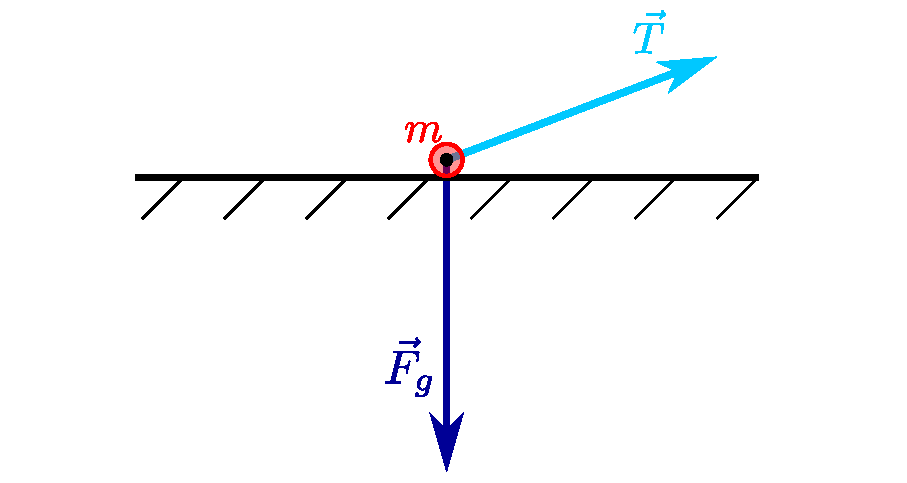
\includegraphics[keepaspectratio=true,width=2.30in]{./how_to_normal_force_and_friction_f01.pdf}
    %\caption{Draw forces other than normal and friction}
    \label{fig:01}
  \end{minipage}
\end{figure}
\FloatBarrier
%-------------------------------------------------------------------------------
\begin{figure}[h!]
  \begin{minipage}[l]{0.70\textwidth}
	{\Large\textsc{Step 2}:} {\large\textsc{Sum these forces}}{\quad}

	Sum all of the forces in Step 1.
	Let's call this $\vec F_{intermediate}$ or just $\vec F_{int}$ for short.

	\vspace{10pt}
	In the example illustrated on the right, $\vec F_{\text{int}}=\vec F_{g} + \vec T$.
  \end{minipage}
  \begin{minipage}[c]{0.25\textwidth}
	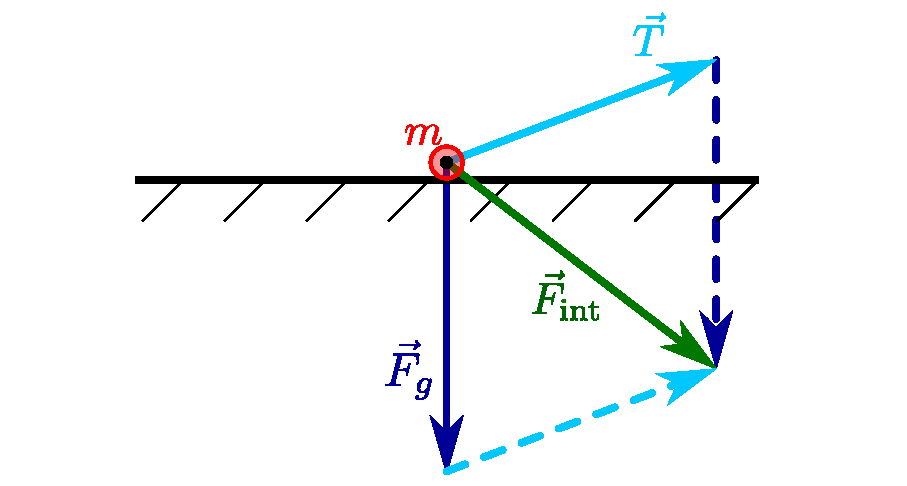
\includegraphics[keepaspectratio=true,width=2.30in]{./how_to_normal_force_and_friction_f02.pdf}
    %\caption{Draw forces other than normal and friction}
    \label{fig:02}
  \end{minipage}
\end{figure}
\FloatBarrier
%{\begin{flushleft}\rule{2in}{0.5pt}\end{flushleft}}
%-------------------------------------------------------------------------------
\begin{figure}[h!]
  \begin{minipage}[l]{0.70\textwidth}
	{\Large\textsc{Step 3}:} {\large\textsc{Break into $\parallel$ and $\perp$ components}}{\quad}

	Break this intermediate result down into its components parallel and perpendicular to the surface.

	\vspace{10pt}
	\textbf{Note}: For Monday's problem (and in the sketches on the right), the parallel ($\parallel$) force components are in the $x$-direction and the perpendicular ($\perp$) components of force is in the $y$-direction.
	\textbf{But this will not, in  general, be true}, so be careful that you pay attention to $\perp$ and $\parallel$ components, \textit{not} necessarily the $x$ and $y$ components.
  \end{minipage}
  \begin{minipage}[l]{0.25\textwidth}
	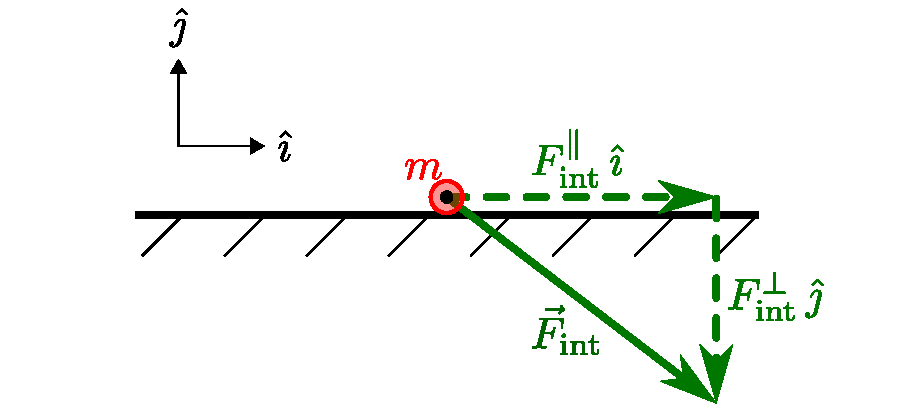
\includegraphics[keepaspectratio=true,width=2.30in]{./how_to_normal_force_and_friction_f03.pdf}
    %\caption{Draw forces other than normal and friction}
    \label{fig:03}
  \end{minipage}
\end{figure}
\FloatBarrier
%{\begin{flushleft}\rule{2in}{0.5pt}\end{flushleft}}
%-------------------------------------------------------------------------------
\begin{figure}[h!]
  \begin{minipage}[l]{0.70\textwidth}
	{\Large\textsc{Step 4}:} {\large\textsc{Find the normal force}}{\quad}

	If there's a component of $\vec F_{int}$ perpendicular to the surface that would push the object through the surface, you have to add in a normal force $\vec n$ to cancel this out.
	%If there object is being accelerated, like if it's resting on the floor of an elevator, then this acceleration, call it $\vec a_{elev}$ will add another ``force'' vector to the problem, which is equal to $m\vec a_{elev}$.

	\vspace{10pt}
	Remember that $\vec n$ is \textit{always} $\perp$ to the surface.
  \end{minipage}
  \begin{minipage}[l]{0.25\textwidth}
	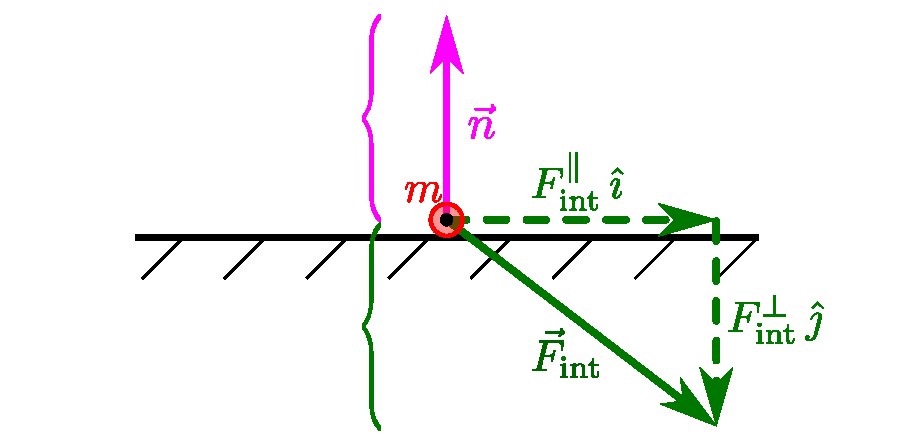
\includegraphics[keepaspectratio=true,width=2.30in]{./how_to_normal_force_and_friction_f04.pdf}
    %\caption{Draw forces other than normal and friction}
    \label{fig:04}
  \end{minipage}
\end{figure}
\FloatBarrier
%{\begin{flushleft}\rule{2in}{0.5pt}\end{flushleft}}
%-------------------------------------------------------------------------------
\begin{figure}[h!]
  \begin{minipage}[l]{0.70\textwidth}
	{\Large\textsc{Step 5}:} {\large\textsc{Find the force due to friction}}{\quad}

	Friction \textit{always} acts in a direction parallel to the surface.
	It can be either kinetic or static friction acting in the problem, where kinetic friction acts when the object is in motion with respect to the surface and static friction acts when the object is at rest relative to the surface.
	In the diagram, I'm using $\vec f$ to generically represent friction, but you can use $\vec f_k$ or $\vec f_s$ to specify kinetic or static friction, respectively.
	%\begin{itemize}
	%  \item \textit{Kinetic} friction is relevant when the object is moving relative to the surface, and it acts in a direction opposite to that relative motion.
	%	In Monday's activity, we assumed that the object was moving to the right relative to the surface, so $\vec f_k$ acted to the left.
	%	
	%	Now that you have the direction of the force, you just need the magnitude.
	%	For kinetic friction, this is $\left\lVert \vec f_k\right\rVert  = \mu_k\left\lVert \vec n\right\rVert $.
	%  \item \textit{Static} friction acts in a direction opposite the component of $\vec F_{\text{int}}$ that is parallel to the surface.
	%	In the drawing on the right, I'm using $F_{\text{int},x}$ as this component, labeled
	%\end{itemize}
  \end{minipage}
  \begin{minipage}[c]{0.25\textwidth}
	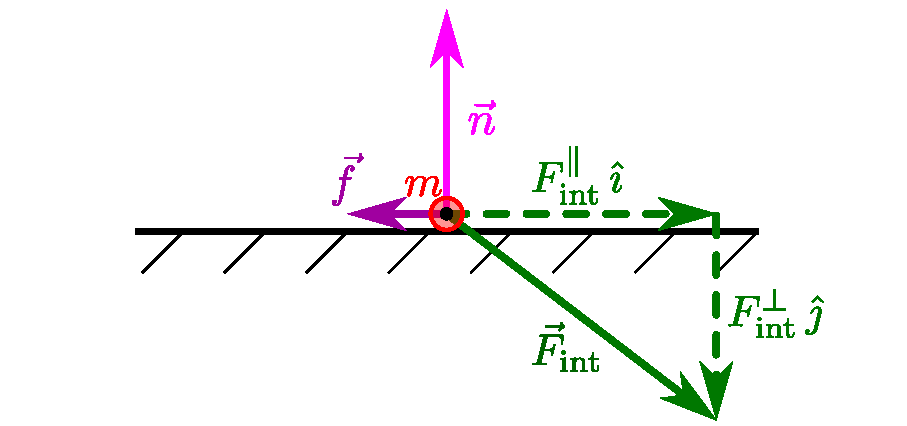
\includegraphics[keepaspectratio=true,width=2.30in]{./how_to_normal_force_and_friction_f05.pdf}
    %\caption{Draw forces other than normal and friction}
    \label{fig:05}
  \end{minipage}
\end{figure}
\FloatBarrier
%{\begin{flushleft}\rule{2in}{0.5pt}\end{flushleft}}
%-------------------------------------------------------------------------------
\begin{figure}[h!]
  \begin{minipage}[l]{0.70\textwidth}
	{\Large\textsc{Step 6}:} {\large\textsc{Draw the free body diagram}}{\quad}

	Now you can draw an accurate representation of the free body diagram.
	A free body diagram must include \textit{all} of the forces that \textit{directly} act on the body. In the example here, those are tension, the gravitational force, the normal force, and the force due to friction.

	\vspace{10pt}
	You could have crudely sketched a free body diagram even before Step~1, but you might have drawn a normal force when there is in fact none and its magnitude (if present) could have been way off. The determination of whether static or kinetic friction is acting, the magnitude of that force, and whether it acts ``left'' or ``right'' with respect to the surface is also, in general, unknown before you've gone through Steps~1--5.
  \end{minipage}
  \begin{minipage}[c]{0.25\textwidth}
	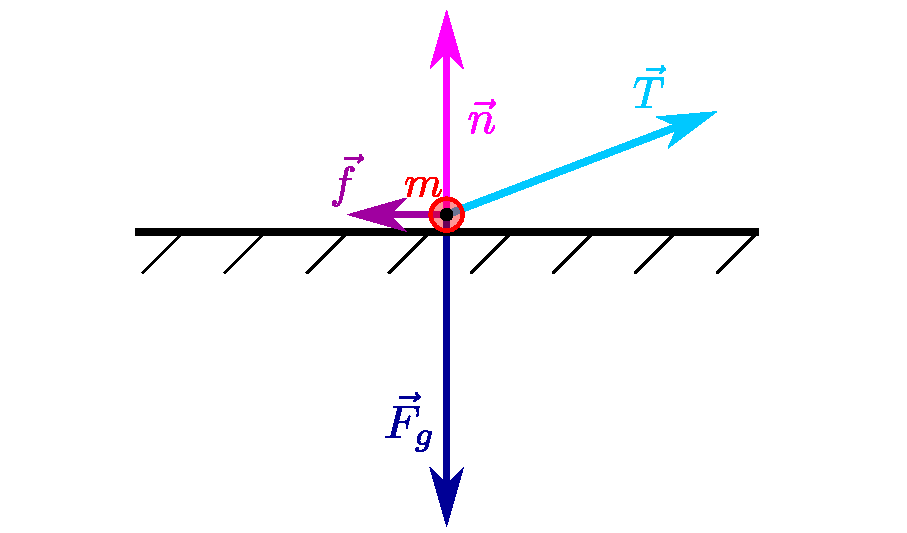
\includegraphics[keepaspectratio=true,width=2.30in]{./how_to_normal_force_and_friction_f06.pdf}
    %\caption{Draw forces other than normal and friction}
    \label{fig:06}
  \end{minipage}
\end{figure}
\FloatBarrier
%{\begin{flushleft}\rule{2in}{0.5pt}\end{flushleft}}
%-------------------------------------------------------------------------------
\begin{figure}[h!]
  \begin{minipage}[l]{0.70\textwidth}
	{\Large\textsc{Step 7}:} {\large\textsc{Find sum of all forces}}{\quad}

	Now that you ``know'' (in quotes since some of the exact magnitudes and the exact direction of the forces might still be unknown\ldots but you labeled them, so I'm calling them ``known'') all of the forces acting, you can find the total force acting on the object, $\vec F_{net}$.

	\vspace{10pt}
	You already found the sum of the forces other than the normal and gravitational forces in Step~2 (and you found the components in Step~3), so it would be acceptable to use that result and then just add to it the normal and friction forces.
	However, to be completely explicit, here I'll re-draw all of the forces and add them together, done by writing the vectors in terms of their components.
%
%	\vspace{10pt}
%	Note that I explicitly write out the signs where magnitudes
  \end{minipage}
  \begin{minipage}[c]{0.25\textwidth}
	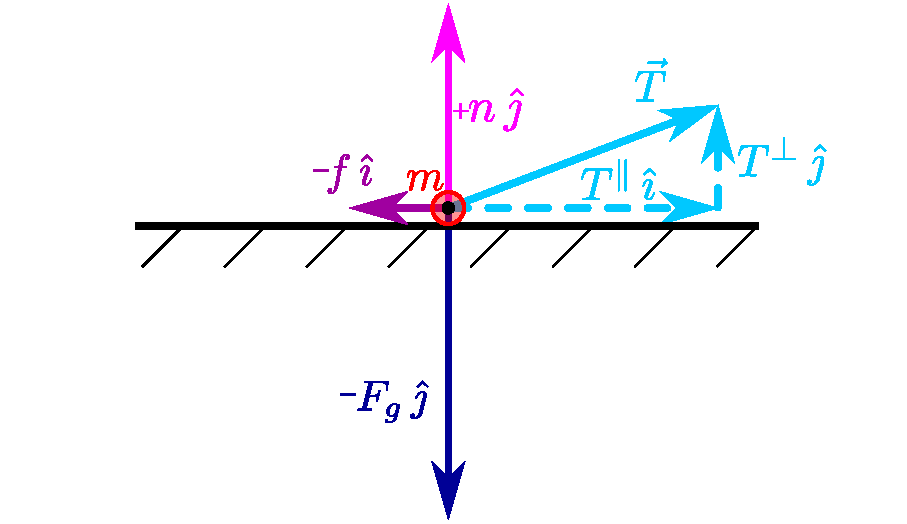
\includegraphics[keepaspectratio=true,width=2.30in]{./how_to_normal_force_and_friction_f07.pdf}
    %\caption{Draw forces other than normal and friction}
    \label{fig:07}
  \end{minipage}
\end{figure}
\FloatBarrier
%{\begin{flushleft}\rule{2in}{0.5pt}\end{flushleft}}
%-------------------------------------------------------------------------------
\begin{figure}[h!]
  \begin{minipage}[l]{0.70\textwidth}
	{\Large\textsc{Step 8}:} {\large\textsc{Find net force perp. to surface}}{\quad}

	Technically, you already know this by now. It's just zero. (Note that if the object is accelerating perpendicular to the surface, like in an elevator, then things change.
	More information for another day.)
  \end{minipage}
  \begin{minipage}[c]{0.25\textwidth}
	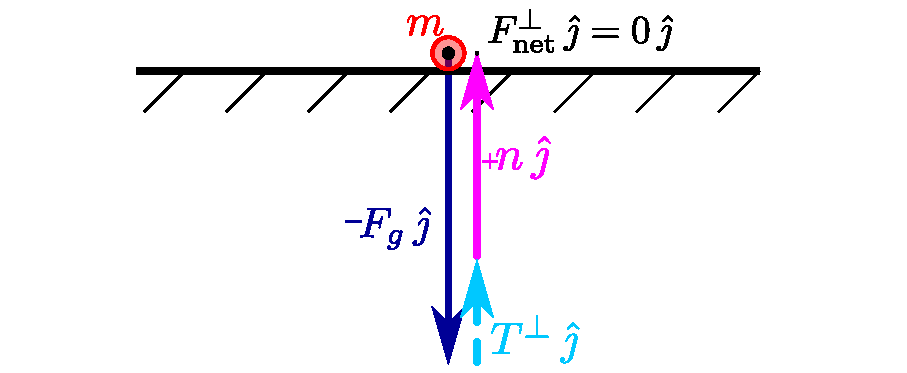
\includegraphics[keepaspectratio=true,width=2.30in]{./how_to_normal_force_and_friction_f08.pdf}
    %\caption{Draw forces other than normal and friction}
    \label{fig:08}
  \end{minipage}
\end{figure}
\FloatBarrier
%{\begin{flushleft}\rule{2in}{0.5pt}\end{flushleft}}
%-------------------------------------------------------------------------------
\begin{figure}[h!]
  \begin{minipage}[l]{0.70\textwidth}
	{\Large\textsc{Step 9}:} {\large\textsc{Find net force parallel to surface}}{\quad}

	The only force component parallel to the surface that you didn't have back in Step~3 was the force due to friction, but now you have that.
	So now you can find the net force parallel to the surface.
  \end{minipage}
  \begin{minipage}[c]{0.25\textwidth}
	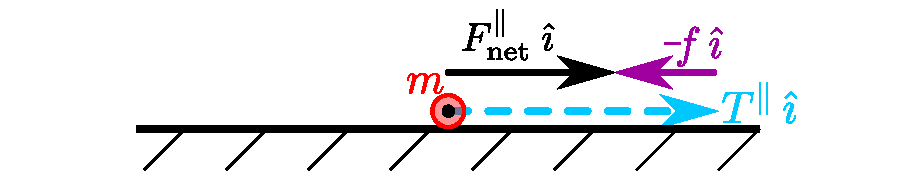
\includegraphics[keepaspectratio=true,width=2.30in]{./how_to_normal_force_and_friction_f09.pdf}
    %\caption{Draw forces other than normal and friction}
    \label{fig:09}
  \end{minipage}
\end{figure}
\FloatBarrier
%{\begin{flushleft}\rule{2in}{0.5pt}\end{flushleft}}
%-------------------------------------------------------------------------------
\begin{figure}[h!]
  \begin{minipage}[l]{0.70\textwidth}
	{\Large\textsc{Step 10}:} {\large\textsc{Apply Newton's 2$^\textsc{nd}$ law}}{\quad}

	You know the net force both perpendicular (Step 8) and parallel (Step 9) to the surface, so you can use Newton's second law written in terms of those components, or you can break down the net force vector (seen at right) into components in another coordinate system.
	Whichever you choose, you can now find the kinematic behavior of the object: $\vec F_{\text{net}}=m\vec a$.
  \end{minipage}
  \begin{minipage}[c]{0.25\textwidth}
	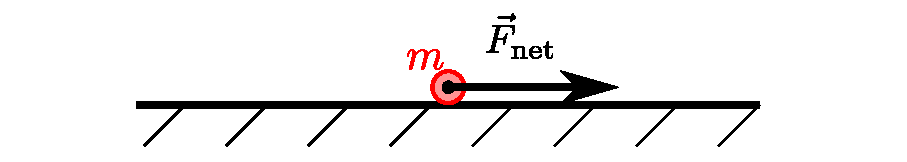
\includegraphics[keepaspectratio=true,width=2.30in]{./how_to_normal_force_and_friction_f10.pdf}
    %\caption{Draw forces other than normal and friction}
    \label{fig:10}
  \end{minipage}
\end{figure}
\FloatBarrier
%{\begin{flushleft}\rule{2in}{0.5pt}\end{flushleft}}
%-------------------------------------------------------------------------------
\begin{figure}[h!]
  \begin{minipage}[l]{0.70\textwidth}
	{\Large\textsc{Net force in context}}{\quad}

	The illustration at right is just to show you the net force in the context of all the forces acting on the object by overlaying $\vec F_{\text{net}}$ on top of the free body diagram from Step~6.
  \end{minipage}
  \begin{minipage}[c]{0.25\textwidth}
	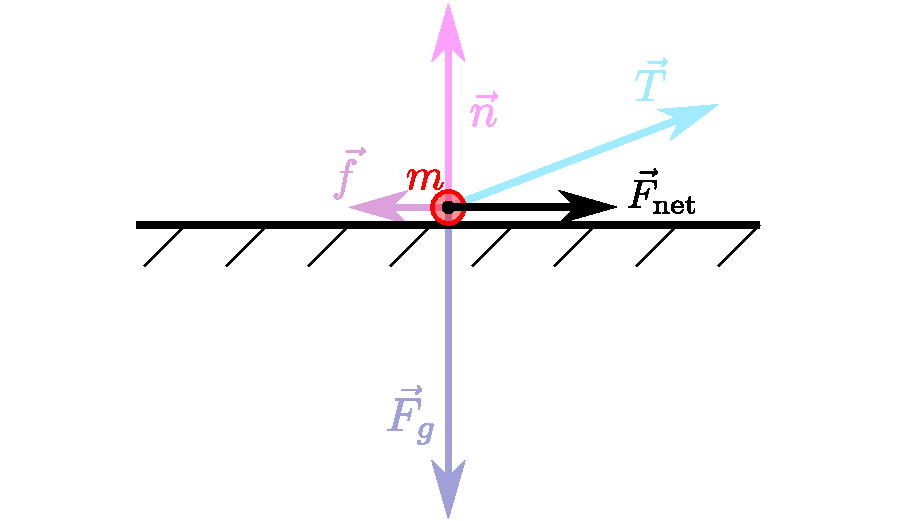
\includegraphics[keepaspectratio=true,width=2.30in]{./how_to_normal_force_and_friction_f11.pdf}
    %\caption{Draw forces other than normal and friction}
    \label{fig:11}
  \end{minipage}
\end{figure}
\FloatBarrier
%-------------------------------------------------------------------------------

%\begin{figure}[h!]
%  \begin{minipage}[l]{0.70\textwidth}
%	{\Large\textsc{Step 1}}{\quad}
%  \end{minipage}
%  \begin{minipage}[c]{0.25\textwidth}
%	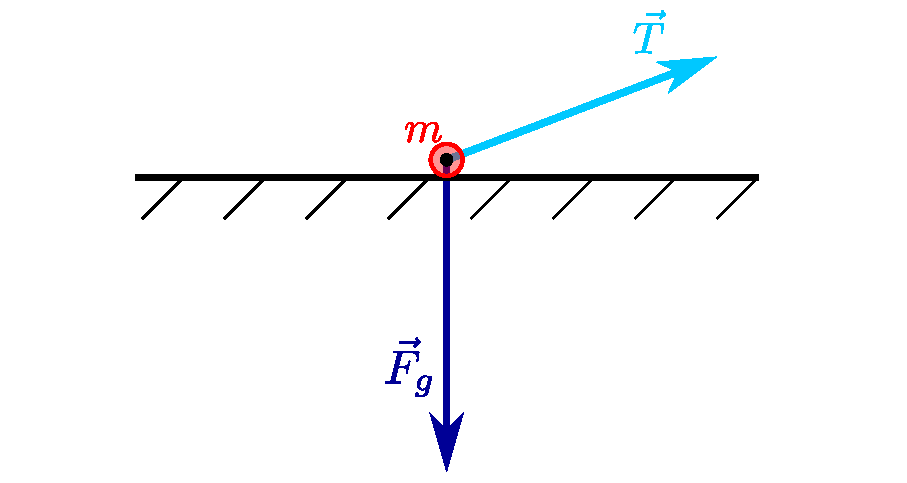
\includegraphics[keepaspectratio=true,width=2.30in]{./how_to_normal_force_and_friction_f01.pdf}
%    %\caption{Draw forces other than normal and friction}
%    \label{fig:01}
%  \end{minipage}
%\end{figure}

\end{document}